\documentclass{ci5652}
\usepackage{graphicx,amssymb,amsmath}
\usepackage[utf8]{inputenc}
\usepackage[spanish]{babel}
\usepackage{hyperref}
\usepackage{subfigure}
\usepackage{paralist}
\usepackage[ruled,vlined,linesnumbered]{algorithm2e}

\graphicspath{ {images/} }

%----------------------- Macros and Definitions --------------------------

% Add all additional macros here, do NOT include any additional files.

% The environments theorem (Theorem), invar (Invariant), lemma (Lemma),
% cor (Corollary), obs (Observation), conj (Conjecture), and prop
% (Proposition) are already defined in the ci5652.cls file.

%----------------------- Title -------------------------------------------

\title{Solución al Problema de la Mochila usando Búsqueda Local}

\author{Marialicia Suárez
        \and
        Sergio Teŕan}

%------------------------------ Text -------------------------------------

\begin{document}
\thispagestyle{empty}
\maketitle


\section*{Resúmen.}
	El problema de la mochila surge cuando hay una asignación de recursos con restricciones de costo. Cada ítem tiene un costo y un valor, se busca obtener el mayor valor posible con un presupuesto dado. El termino \textit{Problema de la mochila} evoca la imagen de un viajero con una mochila de tamaño fijo que debe llenar solo con los ítem mas útiles. Este problema se clasifica como un problema de optimización combinatoria y, computacionalmente, se categoriza como NP-Completo~\cite{c_resumen_01}. Este articulo propone solucionar el problema planteado usando una función heurística de búsqueda local.

	\subsection*{Palabras Clave:}
	Optimización Combinatoria, Metaheuristica, Busqueda Local, Iterativo 

\begin{abstract}
	The Knapsack problem arises when there is an allocation of resources with cost constraints. Each item has a cost and a value, it seeks to obtain the highest value possible with a given budget. The term \textit{Knapsack Problem} evokes the image of a traveler with a backpack fixed size that should be filled only with the most useful item. This problem is classified as a combinatorial optimization problem and, computationally, categorized as NP-Hard. This article proposes to solve the problem raised using a local search heuristic function.
\end{abstract}

	\subsection*{Keywords:}
	Combinatorial Optimization, Metaheuristics, Local Search, Iterative

\section{Introducción.}

	El problema de la mochila (KP por sus siglas en inglés, \textit{Knapsack Problem}) es un problema que ha sido intensamente estudiado por muchos años. El interes en este problema se debe, por una parte a sus aplicaciones directas e indirectas, y por la otra, por ser un campo de prueba que permite ensayar la eficiencia de métodos de solución de búsqueda inteligente en problemas de optimización combinatoria. \\
	Este artículo busca probar la eficiencia de la heurística de optimización combinatoria con búsqueda local utilizando las estrategias de pivoteo \textit{first-improvement} y \textit{best-improvement}.

\section{Busqueda Local.}
	Búsqueda local es un método determinístico y sin memoria, utilizado en muchos otros problemas de optimizacion. Se puede ver como un proceso iterativo que empieza en una solución y la perturba realizando modificaciones locales, buscando en su vecindad por una mejor solución. Si la encuentra, reemplaza su solución actual por la nueva y continua con el proceso, hasta que no se pueda mejorar la solución actual.\\

	\begin{algorithm}
		\DontPrintSemicolon
		\vspace*{0.1cm}
		\KwIn{$S_0$ Solución inicial generada}
		\KwOut{$S$ Optimo local}
		$S = S_0$\;
		\While{$S\ no\ es\ optimo\ local$}{
			$S' \in N_{(S)}$ con $f_{(S)} < f_{(S')}$ (Solución mejor dentro de la vecindad) \;
			$S \leftarrow S' $
		}
		\KwRet{S}
		\vspace*{0.1cm}
		\caption{Busqueda Local}
	\end{algorithm}
		

	El diseño de la vecindad es fundamental para el desepeño del algoritmo. Al hablar de vecindad nos referimos a un conjunto de soluciones cercanas a la solucion actual. Para seleccionar cual solución escoger de esat vecindad, existe distintos acercamientos, siendo posible escoger entre el acercamiento de mejor mejora (\textit{best improvement rule}), primer mejora (\textit{first improvement rule}), aleatorio (\textit{random rule}) entre otros.\\

	\subsection{Estrategias.} 
		La estrategia de pivoteo, puede llegar a ser crucial para el desarrollo del algoritmo, pudiendo generar optimos locales distintos según el caso, y es importante saber escoger cual esatrtegia es la mas adecuada para la funcion objetivo en cuestión.
		En la realizacion de este articulo, se usaron las reglas de pivoteo de \textit{best-improvement} y \textit{random}.
		
		\subsubsection{Mejor Mejora.}
			Bajo esta estrategia, se toma el $S'$ perteneciente al conjunto de soluciones vecinas de $S$ ($S' \in N_{(S)}$) que genera la mejor mejora, es decir, del conjunto de todas las soluciones que superan a la solucion actual, se toma el supremo, y se sustituye $S \leftarrow S'$ para continuar con la iteración.
		
		\subsubsection{Primer Mejora.}
			La estrategia de selección de primer mejora, comienza a recorrer la vecindad $N_(S)$, comparando cada $S'$ que toma con el $S$ actual, al momento que consigue un $S'$ mejor que la solucíón actual, lo toma, para de recorrer el vecindario y sustituye $S \leftarrow S'$	
	
\section{Problema de la Mochila.}
	El problema KP es un problema de optimización combinatoria de formulación sencilla, aunque su resolución es compleja, y que aparece, directamente o como un subproblema en una gran variedad de aplicaciones, incluyendo  planificación de la producción, modelización financiera, muestreo estratificado, planificación de la capacidad de instalaciones, etc.\\
	Además de sus potenciales aplicaciones, el KP es de particular interés por sus características combinatorias y su estructura sencilla, que lo vuelven un problema ideal para el diseño de métodos de búsqueda inteligente. Con el tratamiento del problema KP se pueden evaluar las ventajas y desventajas de estos algoritmos, sobretodo su precisión y rapidez.\\
	El KP es un problema combinatorio que es NP-Completo~\cite{c_KP_01}, que figura en la lista de 21 problemas NP-completos de Karp~\cite{c_KP_04}, por tanto es improbable que, en algún momento, pueda ser encontrado un algoritmo que pueda resolverlo en tiempo polinomial. A pesar de esto, no se cuenta como un porblema fuertemente NP-Completo, por lo que puede ser resuelto en tiempo pseudo-polinomiales particularmente por programación dinámica. Para la realización de este articulo, se implemento una solución con programación dinámica, para considerar como casos optimos, y realizar la comparación de resultados con la heuristica en cuestión (LS). 
	
	\subsection{Formulación.}
	Dado un conjunto de objetos $V = \{ V_1,V_2,\ldots,V_n \}$, donde cada $V_i$ tiene un peso $p_i$ y un beneficio $b_i$ respectivamente, donde $i \in [1,n]$, y dado que se tiene un recipiente (Mochila) con capacidad $C$, el problema KP consiste en determinar la combinación de objetos de $V$ que se agregan en la mochila, de manera que el beneficio obtenido sea el máximo posible, como se puede ver en la Figura 1, donde se tienen 4 items, es decir $V = {(p_1,b_1),(p_2,b_2),(p_3,b_3),(p_4,b_4)}$ y la mochila tiene una capacidad total de C.

 	\begin{figure}[h]
 	\caption{Problema de la Mochila. Como cargar óptimamente la mochila sin rebasar su capacidad máxima.}
	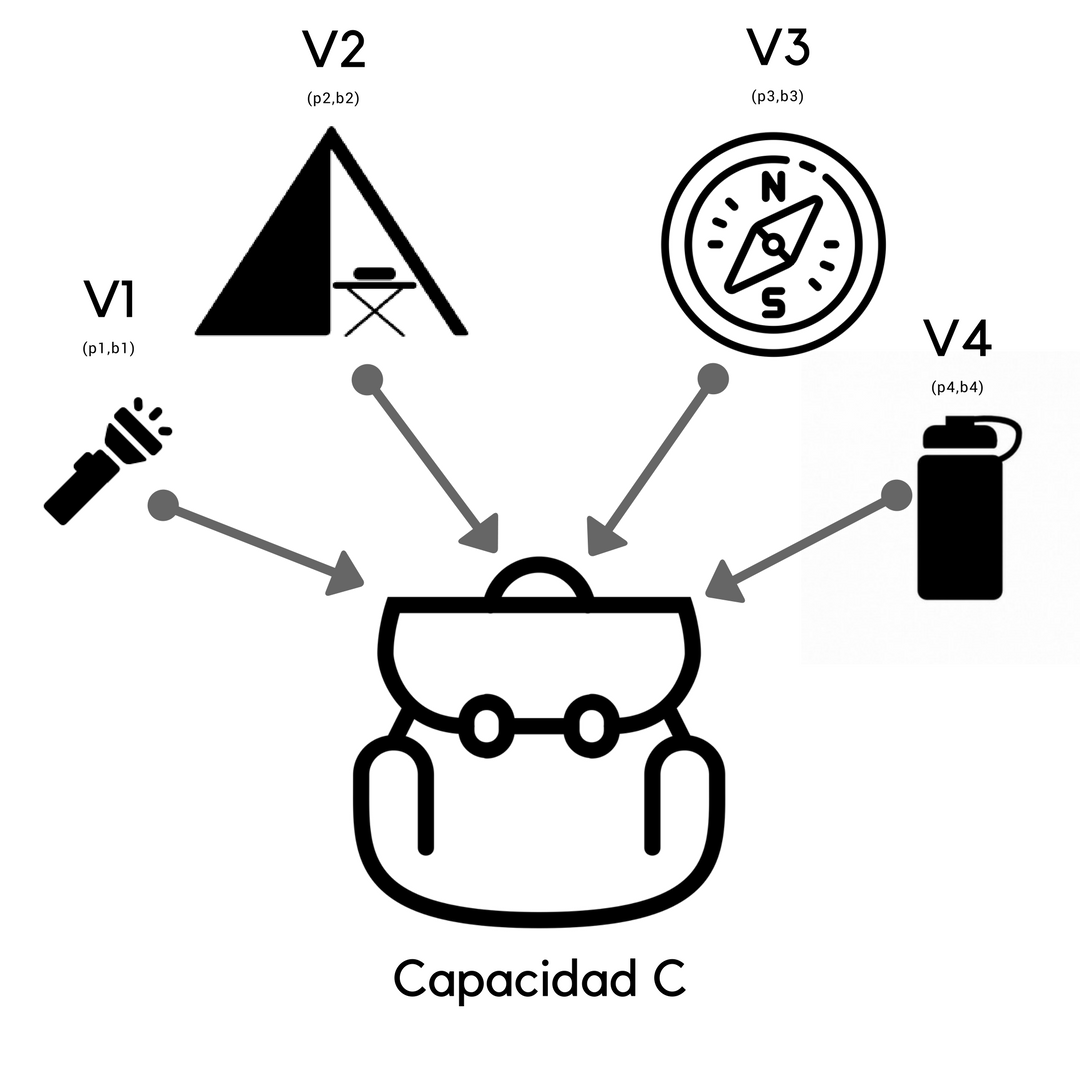
\includegraphics[width=8cm, height=8cm]{KP.png}
	\end{figure}
	\subsection{Función objetivo.}
	En el KP el objetivo es maximizar la suma de los beneficios, por lo que la función objetivo del problema se puede representar como
	$$
		Max \sum_{i=1}^{n} b_i x_i \\
	$$
	Esta funcion esta sujeta a las restricciones de no negatividad y no nulidad ademas de la capacidad maxima, que no puede ser excedida por la sumatoria de los pesos depositados en la mochila.
	$$
		\sum_{i=1}^{n} p_i x_i \leq c
	$$
	$$
	x_i \in \{0,1\};i=1,2,\ldots,n
	$$
	La variable $x_i$ toma el valor de $1$ o $0$ según el elemento $V_i$ pertenece a la combinación dentro de la mochila o no respectivamente.

	\section{Busqueda local para KP.}
	La idea de este estudio es comparar la eficiencia de los procedimientos de busqueda local bajo las estrategias de \textit{best-improvement} y \textit{first-improvement} para resolver el problema KP. Para esta comparación se utilizaron instancias de pruebas generadas de manera aleatoria, y se compararon los resultados de la heuristica de LS, con los resultados obtenidos por la solución de programación dinámica implementada.\\

	\subsection{Estructura de vecindad.}
	Para decidir la forma en la cual se debe determinar el espacio de soluciones $N_{(S)}$ del problema que se aborde, debemos conocer el problema~\cite{c_KP_02}, sin olvidar que el objetivo es maximizar.\\
	Comenzamos partiendo de una solución factible que cumpla con las restricciones del modelo matemático. Los elementos que conforman esta solución son aquellos cuyo peso no sobrepasa el peso soportado por la mochila. La solución inicial también son todos aquellos elementos cuya sumatoria de pesos es menor que la capacidad máxima. Por simplicidad se tomo como $x_i = 0$ para $i = 1\ldots n$.\\
	Para ilustrar la vecindad ~\cite{c_KP_03} (Figura 2), se toma la solución $S = {x_i};i =1\ldots n$, y se consideran los $S'={x_i}$ donde solo una de las $x_i$ cambie su valor ($x_i \in {0,1}$).

 	\begin{figure}[h]
 	\caption{Dado un conjunto de soluciones $U$ la vecindad $N_{(S)}$, indicada por el circulo, se define como los conjuntos $S'$ que solo difieren en un elemento respecto a $S$ (punto dentro de $N_{(S)}$).}
	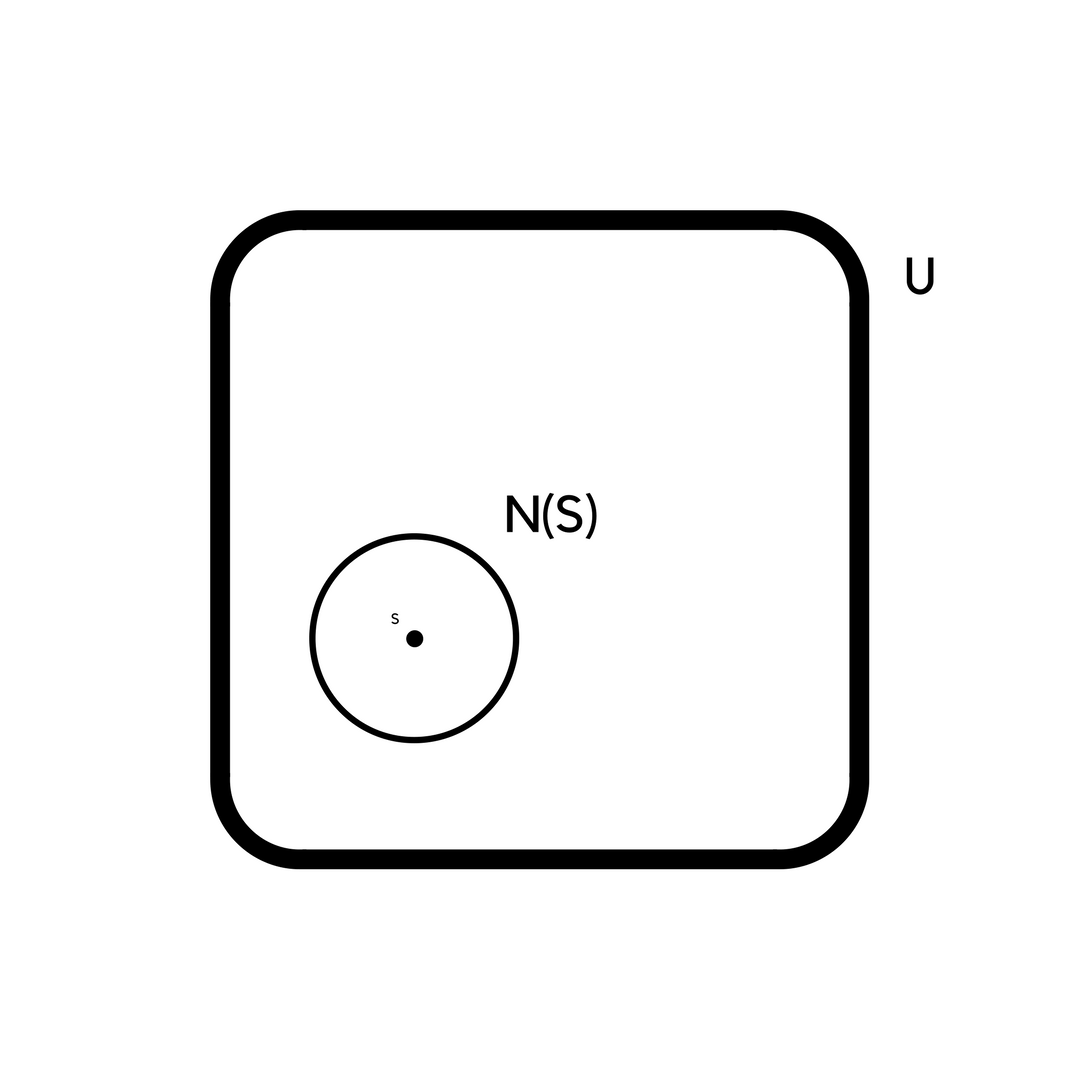
\includegraphics[width=8cm, height=8cm]{Vecindad.png}
	\end{figure}

	Se observa que $S \in U$ y que $N \subset U$. Si se toma un punto $S' \in N_{(S)}$ que represente una mejora respecto a $S$, este se tomara como nueva solución actual. De este modo el metodo de LS va iterando paso a paso desde una solución inicial hacia una solucion que mejore la anterior, que se evalue en la funcion objetivo y que cumpla con todar las restricciones.
	$$
	f(S') \leq f(S)
	$$

\section{Resultados.}
	Para la implementación del algoritmo de programacion dinámica se utilizó el lenguaje de programación Haskell, mientras que para los algoritmos de LS se utilizó el lenguaje de programación Python. Para los casos de uso se utilizaron dos \textit{laptops}, los casos en Haskell se corrieron en un procesador Core i3 con 2Gb de RAM, y para los casos en Python se utilizó tambien un procesador i3 con 4Gb de memoria RAM. Luego de hacer 10 casos de prueba distintos, donde se varian la cantidad de items en $V$ desde 10 hasta 50, se presentan los resultados, comparando los optimos obtenidos para cada caso, al igual que las iteraciones para cada estrategia.\\

 	\begin{figure}[h]
	 	\caption{Tabla 1: Comparacion resultados por caso de prueba}
		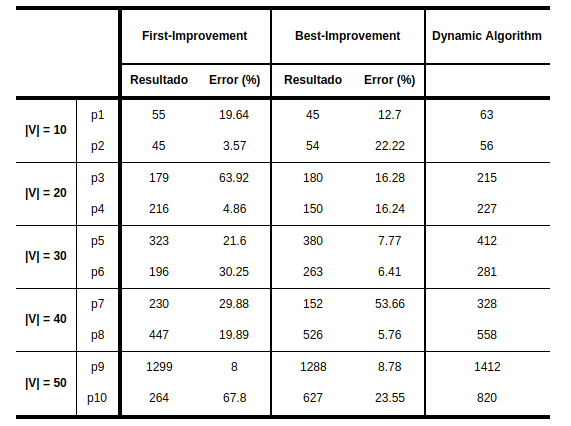
\includegraphics[width=9cm]{errores.png}
	\end{figure}

	En la tabla presentada arriba se observa que tanto el acercamiento por FI como el BI da resultados bastante cercanos al caso de programación dinámica, con errores pequeños, sin embargo, para la mayoria de los casos el error producido por BI es mas pequeño que el error de FI, dando asi resultados generales mas aceptables.\\

 	\begin{figure}[h]
 	\caption{Grafica 1: Regla Mejor Mejora}
	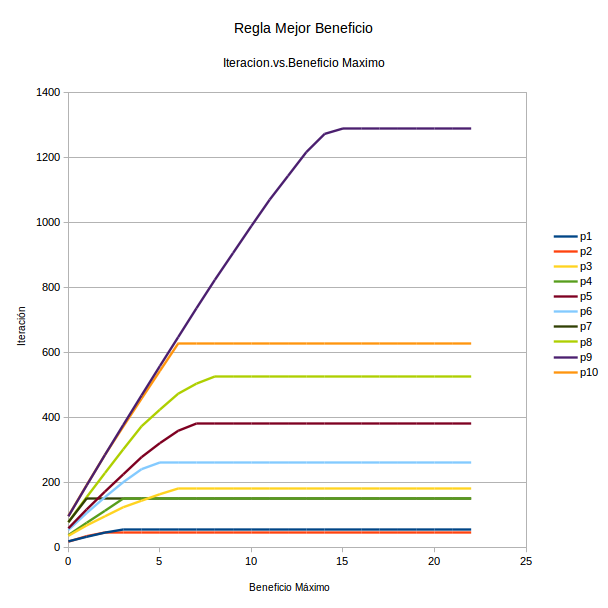
\includegraphics[width=8cm, height=8cm]{best_imp-it-vs-ben_max.png}
	\end{figure}

 	\begin{figure}[h]
 	\caption{Grafica 2: Regla Primer Mejora}
	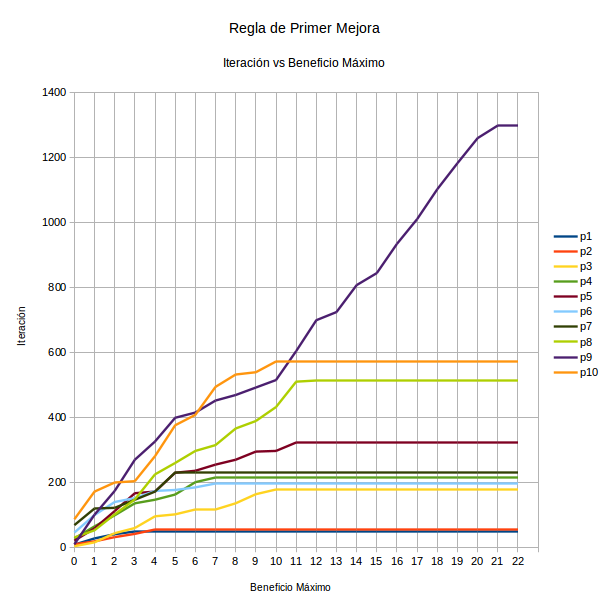
\includegraphics[width=8cm, height=8cm]{first_imp-it-vs-ben_max.png}
	\end{figure}

	En las figuras 4 y 5 se muestran los beneficios maximos en función de la cantidad de iteraciones bajo la estrategia de \textit{best-improvement} (BI) y \textit{first-improvement} (FI) respectivamente, el caso BI describe un crecimiento casi lineal hasta llegar a un valor maximo, mientras que el caso FI tarda mas en crecer. Se puede ver en la tabla 1 (Figura 3) que ambos metodos convergen hacia optimos muy similares, sin embargo, las figuras 4 y 5 evidencia que el metodo BI converge en menos iteraciones que FI para todos los casos.\\
	También se deduce de la Figura 1 que, en la mayoria de los casos, la estrategia de BI produce errores mas pequeños con respecto a la solución de programación dinámica.\\


\section{Discusión y Conclusiones.}
	Se puede apreciar que, a pesar de que ambos metodos generar optimos cercanos a en tiempos mejores que exponencial, el uso de la estrategia de BI genera los mejores resultados en la menor cantidad de iteraciones para la mayoria de los casos, produciendo soluciones con errores pequeños respecto a la soluciíon ofrecida por la programación dinámica.\\

	Es importante destacar que para el problema KP existen casos de prueba que sacan del tiempo pseudo-polinomial al algoritmo de programación dinámica, mientras que el metodo de LS mantiene tiempos pequeños y peudo-lineal, siendo mas eficiente en los casos antes mencionados. Esta eficiencia en el tiempo se mantiene relativamente estable a medida que se aumenta $|V|$ al igual que, si consideramos la solución de Programación Dinámica como la optima, el error de la solución no presenta mayores variaciones.\\

	Para concluir podemos decir que el estudio realizado en este articulo sugiere que el método mas eficiente de LS, para el problema de la Mochila, entre las implementaciones estudiadas, es el que toma como estrategia de pivoteo al regla de Mejor Mejora, ya que es la que en menos iteraciones consigue converger a una solución óptima.

%---------------------------- Bibliography -------------------------------

% Please add the contents of the .bbl file that you generate,  or add bibitem entries manually if you like.
% The entries should be in alphabetical order
\small
\bibliographystyle{abbrv}

\begin{thebibliography}{99}

\bibitem{c_resumen_01}
Papadimitriou, C. H., Steiglitz, K. 
\newblock Combinatorial Optimization: Algorithms and Complexity. 
\newblock {\em New York: Englewood Cliffs}, 1998.


\bibitem{c_KP_01}
M. R. GAREY Y D. S. JOHNSON,
\newblock Computers and Intractability: A Guide to the Theory of NP-Completeness.
\newblock {\em New York: W.H. Freeman}, 1979.

\bibitem{c_KP_02}
Joyanes, A. L., Zahonero, M. I. 
\newblock {Programación en C: Metodología, algoritmos y estructura de datos.}
\newblock{\em México: McGraw-Hill}, 2000.

\bibitem{c_KP_03}
Michaelewicz, Z., Fogel, D. B. 
\newblock {How to Solve it:Modern Heuristics.}
\newblock{\em Berlín: Springer-Verlag}, 2004.

\bibitem{c_KP_04}
Richard M. Karp
\newblock {Reducibility Among Combinatorial Problems.}
\newblock {En R. E. Miller and J. W. Thatcher (editors).}
\newblock { Complexity of Computer Computations.} 
\newblock {\em New York: Plenum. pp. 85-103.}, 1972.

\end{thebibliography}

\end{document}
